\documentclass{llncs}
\usepackage{amsmath,amssymb}
\usepackage{tikz}

\begin{document}

\title{A Purely Definitional Universal Domain}

\author{Brian Huffman}

\institute{Portland State University\\
  \email{brianh@cs.pdx.edu}}

\maketitle

\begin{abstract}
Existing theorem prover tools do not adequately support reasoning
about general recursive datatypes.  Better support for such datatypes
would facilitate reasoning about a wide variety of real-world
programs, including those written in continuation-passing style, that
are beyond the scope of current tools.

This paper introduces a new formalization of a universal domain that
is suitable for modeling general recursive datatypes.  The
construction is purely definitional, introducing no new axioms.
Defining recursive types in terms of this universal domain will allow
a theorem prover to derive strong reasoning principles, with soundness
ensured by construction.
\end{abstract}

\section{Introduction}

One of the main attractions of pure functional languages like Haskell
is that they promise to be easy to reason about.  However, that
promise has not yet been fulfilled.  To illustrate this point, let us
define a couple of datatypes and functions, and try to prove some
simple properties.
\begin{verbatim}
data Cont r a = MkCont ((a -> r) -> r)

mapCont :: (a -> b) -> Cont r a -> Cont r b
mapCont f (MkCont c) = MkCont (\k -> c (k . f))

data Resumption r a = Done a | More (Cont r (Resumption r a))

bind :: Resumption r a -> (a -> Resumption r b) -> Resumption r b
bind (Done x) f = f x
bind (More c) f = More (mapCont (\r -> bind r f) c)
\end{verbatim}

Haskell programmers may recognize type \texttt{Cont} as a standard
continuation monad.  Along with the type definition is a map function
\texttt{mapCont}, for which we expect the functor laws to hold.  By
itself, type \texttt{Cont} is not difficult to work with.  None of the
definitions are recursive, so they can be formalized easily in most
any theorem prover.  Proofs of the functor laws \texttt{mapCont id =
  id} and \texttt{mapCont (f . g) = mapCont f . mapCont g} are
straightforward.

Things get more interesting with the next datatype definition.  Monad
experts might notice that type \texttt{Resumption} is basically a
resumption monad transformer wrapped around a continuation monad.  The
function \texttt{bind} is the monadic bind operation for the
\texttt{Resumption} monad; together with \texttt{Done} as the monadic
unit, we should expect \texttt{bind} to satisfy the monad laws.

The first monad law follows trivially from the definition of
\texttt{bind}.  Instead, let's consider the second monad law (also
known as the right-unit law) which states that \texttt{bind r Done =
  r}.  How can we go about proving this, formally or otherwise?

It might be worthwhile to try case analysis on \texttt{r}, for a
start.  If \texttt{r} is equal to \texttt{Done x}, then from the
definition of \texttt{bind} we have \texttt{bind (Done x) Done = Done
  x}, so the law holds in this case.  Furthermore, if \texttt{r} is
equal to $\bot$, then from the strictness of \texttt{bind} we have
\texttt{bind $\bot$ Done = $\bot$}, so the law also holds for $\bot$.
Finally, we must consider the case when \texttt{r} is equal to
\texttt{More c}.  Using the definition of \texttt{bind} we obtain the
following:
\[
\texttt{bind (More c) Done = More (mapCont (\char '134 r -> bind r Done) c)}
\]
Now, if we could only rewrite the \texttt{bind r Done} on the
right-hand side to \texttt{r}, then we could use the functor identity
law for \texttt{mapCont} to simplify the entire right-hand side to
\texttt{More c}.

Maybe if we had used an appropriate induction rule, then we could have
used an inductive hypothesis to justify rewriting \texttt{bind r Done}
to \texttt{r}.  However, this would have to be a rather unusual
induction rule.  With more ordinary datatypes, the inductive
hypothesis simply assumes that the property being proved holds for an
immediate subterm.  For example, when doing induction over lists, we
get to assume \texttt{P(xs)} in order to show \texttt{P(x : xs)}.
This kind of inductive hypothesis will not work for type
\texttt{Resumption}, because of the indirect recursion in its
definition.

In fact, an induction rule for \texttt{Resumption} appropriate for our
proof does exist, and it is indeed rather unusual.  (The proof of the
second monad law using this induction scheme is left as an exercise
for the reader.)

\begin{equation}
\begin{array}{l}
\mbox{\tt admissible(P)} \\
\mbox{\tt P(undefined)} \\
\mbox{\tt $\forall$x. P(Done x)} \\
\mbox{\tt $\forall$f c. ($\forall$x. P(f x))}
  \longrightarrow \mbox{\tt P(More (mapCont f c))} \\
\hline
\mbox{\tt $\forall$x. P(x)}
\end{array}
\label{eq:induction}
\end{equation}

Possible questions to ask are, ``Where did this rule come from?'' and
``How can we be sure that this rule is correct?''  Many readers are
probably also wondering, ``How did \texttt{mapCont} get in there?''
But for an implementer of theorem proving tools, the most important
question is, ``How can we produce similar induction rules for other
datatypes?''  We will come back to these questions later on.

Unfortunately, a fully mechanized semantics of general recursive
datatypes does not yet exist.  Various theorem provers have facilities
for defining recursive datatypes, but none can properly deal with
datatype definitions like the \texttt{Resumption} type introduced
earlier.  The non--strictly positive recursion causes the definition
to be rejected by both Isabelle/HOL's datatype package and Coq's
inductive definition mechanism.

Of all the currently available theorem proving tools, the
Isabelle/HOLCF domain package is the closest to being able to support
such datatypes.  Since it uses the continuous function space, it is
not limited to strictly positive recursion.  However, the HOLCF domain
package also has some shortcomings.  For example, it does not yet
support indirect recursion properly---it produces induction rules that
are too weak.

Many of its problems stem from the fact that it generates non-trivial
axioms ``on the fly'': For each type definition, the domain package
declares the existence of the new type (without defining it), and
asserts an appropriate type isomorphism and induction rule.  The most
obvious worry with this design is the potential for unsoundness.  For
example, early versions of the domain package could be made to assert
a type isomorphism between a type and its powerset.  On the other
hand, the desire to avoid unsoundness can lead to an implementation
that is too conservative.

In contrast with the current domain package, the Isabelle/HOL
inductive datatype package \cite{paulson97mechanizing} is purely
definitional.  It uses a parameterized universe type, of which new
datatypes are defined as subsets.  Induction rules are not asserted as
axioms; rather, they are proved as theorems.  Using a similar design
for the HOLCF domain package would allow strong reasoning principles
to be generated, with soundness ensured by construction.

The original contributions of this paper are as follows:
\begin{itemize}

\item A new variation on the construction of a universal domain that
  can represent a wide variety of types, including sums, products,
  continuous function space, powerdomains, and recursive types built
  from these.  Universal domain elements are defined in terms of sets
  of natural numbers, using ideal completion---thus the construction
  is suitable for simply-typed, higher-order logic theorem provers.

\item A formalization of this construction in the HOLCF library of the
  Isabelle theorem prover.  The formalization is fully definitional;
  no new axioms are asserted.

\end{itemize}

Section \ref{sec:background} reviews various domain theory concepts
used in the HOLCF formalization.  The construction of the universal
domain type itself, along with embedding and projection functions, are
covered in Section \ref{sec:construction}.  Then Section
\ref{sec:package} describes how the universal domain can be used to
implement a datatype definition package.  After a discussion of
related work in Section \ref{sec:related}, conclusions and directions
for future work are found in Section \ref{sec:conclusion}.

\section{\label{sec:background}Background Concepts}

HOLCF \cite{MuellerNvOS99} is a library of domain theory built on top
of the Isabelle/HOL theorem prover.  HOLCF defines many standard
notions like complete partial orders and continuity; it also defines
standard type constructors like the continuous function space, and
strict sums and products. The remainder of this section is devoted to
some more specialized concepts from HOLCF that support the
formalization of the universal domain.

\subsection{Embedding-Projection Pairs}

Some types can be embedded within other types.  The concept of an
\emph{embedding-projection pair} (often shortened to \emph{ep-pair})
formalizes this notion.  Let $A$ and $B$ be cpos, and $e : A
\rightarrow B$ and $p : B \rightarrow A$ be continuous functions.
Then $e$ and $p$ are an ep-pair if $p \circ e = \mathrm{Id}_A$ and $e
\circ p \sqsubseteq \mathrm{Id}_B$.  The existence of such an ep-pair
means that type $A$ can be embedded within type $B$.

\begin{figure}
\begin{verbatim}
data Shrub = Node Shrub Shrub | Tip
data Tree = Branch Tree Tree | Leaf | Twig

embed :: Shrub -> Tree
embed (Node l r) = Branch (embed l) (embed r)
embed Tip = Twig

project :: Tree -> Shrub
project (Branch l r) = Node (project l) (project r)
project Leaf = undefined
project Twig = Tip

deflate :: Tree -> Tree
deflate (Branch l r) = Branch (deflate l) (deflate r)
deflate Leaf = undefined
deflate Twig = Twig
\end{verbatim}
\caption{\label{fig:ep-pair}Embedding-projection pairs and deflations
  in Haskell.  Function \texttt{deflate} is equal to the composition
  of functions \texttt{embed} and \texttt{project}.}
\end{figure}

Figure~\ref{fig:ep-pair} shows an example in Haskell, where the the
type \texttt{Shrub} is embedded into the larger type \texttt{Tree}.
If we embed a value from type \texttt{Shrub} into type \texttt{Tree},
and then project back out, then we always get back the same value.  In
other words, for all \texttt{s} of type \texttt{Shrub}, we have
\texttt{project (embed s) $=$ s}.  On the other hand, if we start with
\texttt{t} of type \texttt{Tree}, project out to type \texttt{Shrub},
then embed back into type \texttt{Tree}, we may or may not get back
the same value we started with.  If \texttt{t} contains no
\texttt{Leaf} constructors at all, then we have \texttt{embed (project
  t) $=$ t}.  Otherwise, what we end up with is basically a tree with
all its leaves stripped off---each \texttt{Leaf} constructor is
replaced with $\bot$.

\subsection{Deflations}

Cpo types may contain other cpos as subsets.  A
\emph{deflation}\footnote{My usage of \emph{deflation} follows Gunter
  \cite{gunter85thesis}.  Many authors use the term \emph{projection}
  to refer to the same concept, but I prefer \emph{deflation} because
  it avoids confusion with the second half of an ep-pair.} is a way to
encode such a sub-cpo as a continuous function.  Let $B$ be a cpo, and
$d : B \rightarrow B$ be a continuous function.  Then $d$ is a
deflation if $d \circ d = d \sqsubseteq \mathrm{Id}_B$.  The image set
of deflation $d : B \rightarrow B$ gives a sub-cpo of $B$.

Essentially, a deflation is a \emph{value} that represents a
\emph{type}.  For example, the function \texttt{deflate} in
Fig.~\ref{fig:ep-pair} is a deflation; its image set consists of
exactly those values of type \texttt{Tree} that contain no
\texttt{Leaf} constructors.  Note that while the the definition of
\texttt{deflate} does not mention type \texttt{Shrub} at all, its
image set is isomorphic to type \texttt{Shrub}: In other words,
\texttt{deflate} (a function value) is a representation of
\texttt{Shrub} (a type).

While types can be represented by deflations, type \emph{constructors}
(which are like functions from types to types) can be represented as
functions from deflations to deflations.  For example, the
\texttt{map} function represents Haskell's list type constructor:
While \texttt{deflate} is a deflation on type \texttt{Tree} that
represents type \texttt{Shrub}, \texttt{map deflate} is a deflation on
type \texttt{[Tree]} that represents type \texttt{[Shrub]}.

Deflations and ep-pairs are closely related.  Given an ep-pair $(e, p)$
from cpo $A$ into cpo $B$, the composition $e \circ p$ is a deflation
on $B$ whose image set is isomorphic to $A$.  Conversely, every
deflation $d : B \rightarrow B$ also gives rise to an ep-pair.  Define
the cpo $A$ to be the image set of $d$; also define $e$ to be the
inclusion map from $A$ to $B$, and define $p = d$.  Then $(e, p)$ is
an embedding-projection pair.  So saying that there exists an ep-pair
from A to B is equivalent to saying that there exists a deflation on B
whose image set is isomorphic to A.

Finally we are ready to talk about what it means for a cpo to be a
universal domain.  A cpo $U$ is universal for a class of cpos, if for
every cpo $D$ in the class, there exists an ep-pair from $D$ into $U$.
Equivalently, for every $D$ there must exist a deflation on $U$ with
an image set isomorphic to $D$.

\subsection{Algebraic and Bifinite Cpos}

Lazy recursive datatypes often have infinite as well as finite
values.\footnote{\emph{Compactness} is the precise technical version
  of the more intuitive concept of \emph{finiteness}.  The concepts do
  not necessarily coincide: For example, in a cpo of ordinals, $\omega
  + 1$ is compact but not finite.  In the context of recursive
  datatypes, however, the concepts are equivalent.}  For example, we
can define a datatype of recursive lazy lists of booleans:
\begin{verbatim}
data BoolList = Nil | Cons Bool BoolList
\end{verbatim}
Finite values of type \texttt{BoolList} include total values like
\texttt{Cons False Nil}, and \texttt{Cons True (Cons False Nil)},
along with partial finite values like \texttt{Cons False undefined}.
On the other hand, recursive definitions can yield infinite values:
\begin{verbatim}
trues :: BoolList
trues = Cons True trues
\end{verbatim}

One way to characterize the set of finite values is in terms of an
\texttt{approx} function, defined below.  The function \texttt{approx}
is similar to the standard list function \texttt{take} that we all
know and love, except that \texttt{approx 0} returns $\bot$ instead of
\texttt{Nil}.  (This makes each \texttt{approx n} into a deflation.)
A value \texttt{xs} of type \texttt{BoolList} is finite if and only if
there exists some \texttt{n} such that \texttt{approx n xs $=$ xs}.
\begin{verbatim}
approx :: Int -> BoolList -> BoolList
approx 0 xs = undefined
approx n Nil = Nil
approx n (Cons x xs) = Cons x (approx (n-1) xs)
\end{verbatim}

The function \texttt{approx} is so named because for any input value
\texttt{xs} it generates a sequence of finite approximations to
\texttt{xs}.  For example, the first few approximations to
\texttt{trues} are $\bot$, \texttt{Cons True $\bot$}, \texttt{Cons
  True (Cons True $\bot$)}, and so on.  Each is finite, but the least
upper bound of the sequence is the infinite value \texttt{trues}.
This property of a cpo, where every infinite value can be written as
the least upper bound of a chain of finite values, is called
\emph{algebraicity}.  Thus \texttt{BoolList} is an \emph{algebraic
  cpo}.

The sequence of deflations \texttt{approx n} is a chain of functions
whose least upper bound is the identity function.  In terms of image
sets, we have a sequence of partial orders whose limit is the whole
type \texttt{BoolList}.

A further property of \texttt{approx} which may not be immediately
apparent is that for any \texttt{n}, the image of \texttt{approx n} is
a finite set.  This means that image sets of \texttt{approx n} yield a
sequence of \emph{finite} partial orders.  As a limit of finite
partial orders, we say that type \texttt{BoolList} is a
\emph{bifinite} cpo.  More precisely, as a limit of \emph{countably
  many} finite partial orders, \texttt{BoolList} is an
\emph{omega}-bifinite cpo.\footnote{``SFP domain'' is another name,
introduced by Plotkin \cite{plotkin76powerdomain}, that is used for
the same concept---the name stands for Sequence of Finite Posets.}

The omega-bifinites are a useful class of cpos because bifiniteness is
preserved by all of the type constructors defined in HOLCF.
Furthermore, all Haskell datatypes are omega-bifinite.  Basically any
type constructor that preserves finiteness will preserve bifiniteness
as well.  More details about the formalization of omega-bifinite
domains in HOLCF can be found in \cite{huffman08powerdomain}.

\subsection{Ideal Completion and Continuous Extensions}

In an algebraic cpo the set of finite elements, together with the
ordering relation on them, completely determines the structure of the
entire cpo.  We say that the set of finite elements forms a
\emph{basis} for the cpo, and the entire cpo is a \emph{completion} of
the basis.

Given a basis $B$ with ordering relation ($\preceq$), we can
reconstruct the whole algebraic cpo. The standard process for doing
this is called \emph{ideal completion}, and it is done by considering
the set of ideals over the basis.

\begin{definition}
A set $S$ is an \emph{ideal} with respect to partial preorder relation
$(\preceq)$ if it has the following properties:
\begin{itemize}
\item $S$ is nonempty: $\exists x.\, x\in S$
\item $S$ is downward-closed: $\forall x\, y.\, x\preceq y\longrightarrow y\in S\longrightarrow x\in S$
\item $S$ is directed (i.e. has an upper bound for any pair of elements):\\
 $\forall x\, y.\, x\in S\longrightarrow y\in S\longrightarrow(\exists z.\, z\in S\wedge x\preceq z\wedge y\preceq z)$
\end{itemize}
A \emph{principal} \emph{ideal} is an ideal of the form $\{y \mid y\preceq x\}$
for some $x$, denoted $\downarrow\! x$.
\end{definition}
The set of all ideals over $\left\langle B,\preceq\right\rangle $ is
denoted $\mathrm{Idl}(B)$; when ordered by subset inclusion,
$\mathrm{Idl}(B)$ forms an algebraic cpo. The compact elements of
$\mathrm{Idl}(B)$ are exactly those represented by principal ideals.

Note that the relation $(\preceq)$ does not need to be antisymmetric.
For $x$ and $y$ that are equivalent (that is, both $x\preceq y$
and $y\preceq x$) the principal ideals $\downarrow\! x$ and $\downarrow\! y$
are equal. This means that the ideal completion construction automatically
takes care of quotienting by the equivalence induced by $(\preceq)$.

Just as the structure of an algebraic cpo is completely determined by
its basis, a continuous function from an algebraic cpo to another type
is completely determined by its action on basis elements.  This
suggests a method for defining continuous functions over ideal
completions: First, define a function from the basis $B$ to a cpo $C$
such that $f$ is monotone, i.e.  $x\preceq y$ implies $f(x)\sqsubseteq
f(y)$.  Then there exists a unique continuous function
$\widehat{f}:\mathrm{Idl}(B)\rightarrow C$ that agrees with $f$ on
principal ideals, i.e. for all $x$, $\widehat{f}(\downarrow\!
x)=f(x)$.  We say that $\widehat{f}$ is the \emph{continuous
  extension} of $f$.

In the next section, all of the constructions related to the universal
domain will be done in terms of basis values: The universal domain
itself will be defined using ideal completion, and the embedding and
projection functions will be defined as continuous extensions.

HOLCF includes a formalization of ideal completion and continuous
extensions, which was created to support the definition of
powerdomains \cite{huffman08powerdomain}.


\section{\label{sec:construction}Construction of the Universal Domain}

Informally, an \emph{omega-bifinite domain} is a cpo that can be
written as the limit of a sequence of finite partial orders.  This
section describes how to construct a \emph{universal} omega-bifinite
domain $U$, along with an ep-pair from another arbitrary
omega-bifinite domain $D$ into $U$.  The general strategy is as
follows:
\begin{itemize}
\item From the bifinite structure of $D$, obtain a sequence of finite
  posets $P_n$ whose limit is $D$.
\item Following Gunter \cite{gunter87universal}, decompose the
  sequence $P_n$ further into a sequence of \emph{increments} that
  insert new elements one at a time.
\item Construct the universal domain $U$ using ideal completion, such
  that it can encode any increment.
\item Define the embedding and projection functions between $D$ and
  $U$ using continuous extension, in terms of their action on basis
  elements.
\end{itemize}

\subsection{Building a Sequence of Increments}

Any omega-bifinite domain $D$ can be represented as the limit of a
sequence of finite posets, with embedding-projection pairs between
each successive pair.  Figure~\ref{fig:posets} shows the first few
posets from one such sequence.

\begin{figure}
\begin{center}
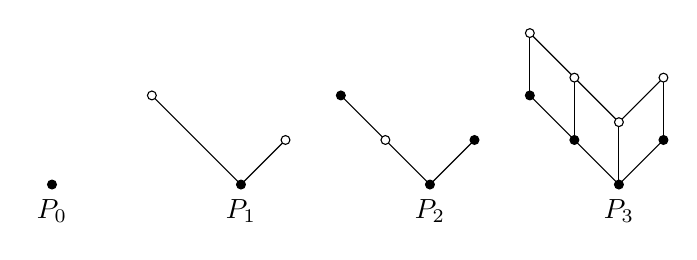
\begin{tikzpicture}[scale=0.8]
  \begin{scope}[rotate=45]
    \filldraw (0,0) circle (2pt);
    \draw (-0.3, -0.3) node {$P_0$};
  \end{scope}
  \begin{scope}[xshift=3cm,rotate=45]
    \draw (0.0, 0.0) -- (0.0, 2.0);
    \draw (0.0, 0.0) -- (1.0, 0.0);
    \filldraw[fill=black] (0.0, 0.0) circle (2pt);
    \filldraw[fill=white] (0.0, 2.0) circle (2pt);
    \filldraw[fill=white] (1.0, 0.0) circle (2pt);
    \draw (-0.3, -0.3) node {$P_1$};
  \end{scope}
  \begin{scope}[xshift=6cm,rotate=45]
    \draw (0.0, 0.0) -- (0.0, 2.0);
    \draw (0.0, 0.0) -- (1.0, 0.0);
    \filldraw[fill=black] (0.0, 0.0) circle (2pt);
    \filldraw[fill=black] (0.0, 2.0) circle (2pt);
    \filldraw[fill=black] (1.0, 0.0) circle (2pt);
    \filldraw[fill=white] (0.0, 1.0) circle (2pt);
    \draw (-0.3, -0.3) node {$P_2$};
  \end{scope}
  \begin{scope}[xshift=9cm,rotate=45]
    \draw (0.0, 2.0) -- (0.0, 0.0) -- (1.0, 0.0);
    \draw (0.7, 2.7) -- (0.7, 0.7) -- (1.7, 0.7);
    \draw (0.0, 2.0) -- (0.7, 2.7);
    \draw (0.0, 1.0) -- (0.7, 1.7);
    \draw (0.0, 0.0) -- (0.7, 0.7);
    \draw (1.0, 0.0) -- (1.7, 0.7);
    \filldraw[fill=black] (0.0, 0.0) circle (2pt);
    \filldraw[fill=black] (0.0, 2.0) circle (2pt);
    \filldraw[fill=black] (0.0, 1.0) circle (2pt);
    \filldraw[fill=black] (1.0, 0.0) circle (2pt);
    \filldraw[fill=white] (0.7, 0.7) circle (2pt);
    \filldraw[fill=white] (0.7, 2.7) circle (2pt);
    \filldraw[fill=white] (0.7, 1.7) circle (2pt);
    \filldraw[fill=white] (1.7, 0.7) circle (2pt);
    \draw (-0.3, -0.3) node {$P_3$};
  \end{scope}
\end{tikzpicture}
\end{center}
\caption{\label{fig:posets}A sequence of finite posets. Each $P_n$ can
  be embedded into $P_{n+1}$; black nodes indicate the range of the
  embedding function.}
\end{figure}

In each step along the chain, each new poset $P_{n+1}$ is larger than
the previous $P_n$ by some finite amount; the structure of $P_{n+1}$
has $P_n$ embedded within it, but it has some new elements as well.

An ep-pair between finite posets $P$ and $P'$, where $P'$ has exactly
one more element than $P$, is called an \emph{increment} (terminology
due to Gunter \cite{gunter92semantics}).  In Fig.~\ref{fig:posets},
the embedding of $P_1$ into $P_2$ is an example of an increment.

The strategy for embedding a bifinite domain into the universal domain
is built around increments.  The universal domain is designed so that
if a finite partial order $P$ is representable (i.e. by a deflation),
and there is an increment from $P$ to $P'$, then $P'$ will also be
representable.

For all embeddings from $P_n$ to $P_{n+1}$ that add more than one new
value, we will need to decompose the single large embedding into a
sequence of smaller increments.  The challenge, then, is to determine
which order the new elements should be inserted.  The order matters:
Adding elements in the wrong order can cause problems, as shown in
Fig.~\ref{fig:order}.

\begin{figure}
\begin{center}
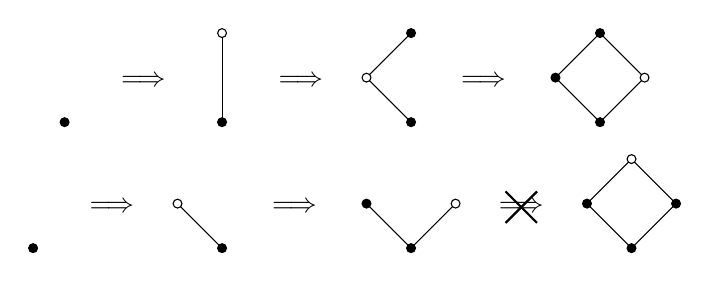
\begin{tikzpicture}[scale=0.8]
  \begin{scope}[xshift=0cm,rotate=45]
    \filldraw (0,0) circle (2pt);
  \end{scope}
  \begin{scope}[xshift=3.0cm,rotate=45]
    \draw (0.0, 0.0) -- (0.0, 1.0);
    \filldraw[fill=black] (0.0, 0.0) circle (2pt);
    \filldraw[fill=white] (0.0, 1.0) circle (2pt);
  \end{scope}
  \begin{scope}[xshift=6.0cm,rotate=45]
    \draw (0.0, 0.0) -- (0.0, 1.0);
    \draw (0.0, 0.0) -- (1.0, 0.0);
    \filldraw[fill=black] (0.0, 0.0) circle (2pt);
    \filldraw[fill=black] (0.0, 1.0) circle (2pt);
    \filldraw[fill=white] (1.0, 0.0) circle (2pt);
  \end{scope}
  \begin{scope}[xshift=9.5cm,rotate=45]
    \draw (0.0, 1.0) -- (0.0, 0.0) -- (1.0, 0.0);
    \draw (0.0, 1.0) -- (1.0, 1.0) -- (1.0, 0.0);
    \filldraw[fill=black] (0.0, 0.0) circle (2pt);
    \filldraw[fill=black] (0.0, 1.0) circle (2pt);
    \filldraw[fill=black] (1.0, 0.0) circle (2pt);
    \filldraw[fill=white] (1.0, 1.0) circle (2pt);
  \end{scope}
  \draw (1.25, 0.65) node {$\Longrightarrow$};
  \draw (4.15, 0.65) node {$\Longrightarrow$};
  \draw (7.75, 0.65) node {$\Longrightarrow$};
  \draw[thick] (7.5, 0.4) -- (8.0, 0.9);
  \draw[thick] (7.5, 0.9) -- (8.0, 0.4);

  \begin{scope}[xshift=0.5cm,yshift=2cm]
  \begin{scope}[xshift=0cm,rotate=45]
    \filldraw (0,0) circle (2pt);
  \end{scope}
  \begin{scope}[xshift=2.5cm,rotate=45]
    \draw (0.0, 0.0) -- (1.0, 1.0);
    \filldraw[fill=black] (0.0, 0.0) circle (2pt);
    \filldraw[fill=white] (1.0, 1.0) circle (2pt);
  \end{scope}
  \begin{scope}[xshift=5.5cm,rotate=45]
    \draw (0.0, 0.0) -- (0.0, 1.0) -- (1.0, 1.0);
    \filldraw[fill=black] (0.0, 0.0) circle (2pt);
    \filldraw[fill=black] (1.0, 1.0) circle (2pt);
    \filldraw[fill=white] (0.0, 1.0) circle (2pt);
  \end{scope}
  \begin{scope}[xshift=8.5cm,rotate=45]
    \draw (0.0, 0.0) -- (0.0, 1.0) -- (1.0, 1.0);
    \draw (0.0, 0.0) -- (1.0, 0.0) -- (1.0, 1.0);
    \filldraw[fill=black] (0.0, 0.0) circle (2pt);
    \filldraw[fill=black] (1.0, 1.0) circle (2pt);
    \filldraw[fill=black] (0.0, 1.0) circle (2pt);
    \filldraw[fill=white] (1.0, 0.0) circle (2pt);
  \end{scope}
  \draw (1.25, 0.65) node {$\Longrightarrow$};
  \draw (3.75, 0.65) node {$\Longrightarrow$};
  \draw (6.65, 0.65) node {$\Longrightarrow$};
  \end{scope}
\end{tikzpicture}
\end{center}
\caption{\label{fig:order} The right (top) and wrong (bottom) way to
  order insertions.  No ep-pair exists between the 3-element and
  4-element posets on the bottom row.}
\end{figure}

To describe the position of a newly-inserted element, it will be
helpful to invent some terminology.  The set of elements \emph{above}
the new element will be known as its \emph{superiors}.  An element
immediately \emph{below} the new element will be known as its
\emph{subordinate}.

In order for the insertion of a new element to be a valid increment,
it must have exactly one subordinate.  The subordinate indicates the value
that the increment's projection maps the new value onto.

With the four-element poset in the Fig.~\ref{fig:order}, it is not
possible to insert the top element last.  The reason is that the
element has two subordinates: If a projection function maps the new
element to one, the ordering relation with the other will not be
preserved.  Thus a monotone projection does not exist.

A strategy for successfully avoiding such situations is to always
insert maximal elements first \cite[\S5]{gunter87universal}.
Fig.~\ref{fig:increments} shows this strategy in action.  Notice that
the number of superiors varies from step to step, but each inserted
element always has exactly one subordinate.  To maintain this
invariant, the least of the four new values must be inserted last.

\begin{figure}
\begin{center}
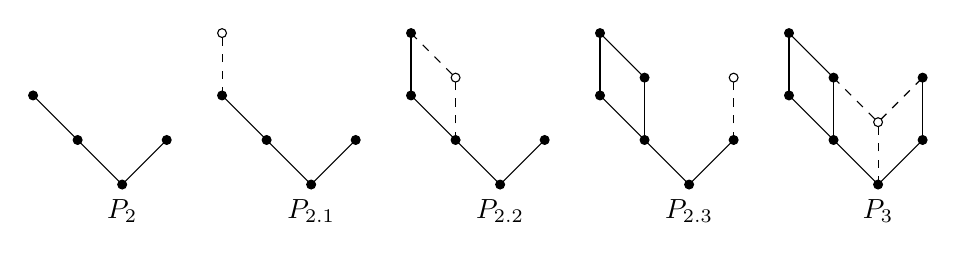
\begin{tikzpicture}[scale=0.8]
  \begin{scope}[xshift=0cm,rotate=45]
    \draw (0.0, 2.0) -- (0.0, 0.0) -- (1.0, 0.0);
    \filldraw[fill=black] (0.0, 0.0) circle (2pt);
    \filldraw[fill=black] (0.0, 2.0) circle (2pt);
    \filldraw[fill=black] (0.0, 1.0) circle (2pt);
    \filldraw[fill=black] (1.0, 0.0) circle (2pt);
    \draw (-0.3, -0.3) node {$P_2$};
  \end{scope}
  \begin{scope}[xshift=3cm,rotate=45]
    \draw (0.0, 2.0) -- (0.0, 0.0) -- (1.0, 0.0);
    \draw[dashed] (0.0, 2.0) -- (0.7, 2.7);
    \filldraw[fill=black] (0.0, 0.0) circle (2pt);
    \filldraw[fill=black] (0.0, 2.0) circle (2pt);
    \filldraw[fill=black] (0.0, 1.0) circle (2pt);
    \filldraw[fill=black] (1.0, 0.0) circle (2pt);
    \filldraw[fill=white] (0.7, 2.7) circle (2pt);
    \draw (-0.3, -0.3) node {$P_{2.1}$};
  \end{scope}
  \begin{scope}[xshift=6cm,rotate=45]
    \draw (0.0, 2.0) -- (0.0, 0.0) -- (1.0, 0.0);
    \draw (0.0, 2.0) -- (0.7, 2.7);
    \draw[dashed] (0.7, 2.7) -- (0.7, 1.7);
    \draw[dashed] (0.0, 1.0) -- (0.7, 1.7);
    \filldraw[fill=black] (0.0, 0.0) circle (2pt);
    \filldraw[fill=black] (0.0, 2.0) circle (2pt);
    \filldraw[fill=black] (0.0, 1.0) circle (2pt);
    \filldraw[fill=black] (1.0, 0.0) circle (2pt);
    \filldraw[fill=black] (0.7, 2.7) circle (2pt);
    \filldraw[fill=white] (0.7, 1.7) circle (2pt);
    \draw (-0.3, -0.3) node {$P_{2.2}$};
  \end{scope}
  \begin{scope}[xshift=9cm,rotate=45]
    \draw (0.0, 2.0) -- (0.0, 0.0) -- (1.0, 0.0);
    \draw (0.0, 2.0) -- (0.7, 2.7);
    \draw (0.7, 2.7) -- (0.7, 1.7);
    \draw (0.0, 1.0) -- (0.7, 1.7);
    \draw[dashed] (1.0, 0.0) -- (1.7, 0.7);
    \filldraw[fill=black] (0.0, 0.0) circle (2pt);
    \filldraw[fill=black] (0.0, 2.0) circle (2pt);
    \filldraw[fill=black] (0.0, 1.0) circle (2pt);
    \filldraw[fill=black] (1.0, 0.0) circle (2pt);
    \filldraw[fill=black] (0.7, 2.7) circle (2pt);
    \filldraw[fill=black] (0.7, 1.7) circle (2pt);
    \filldraw[fill=white] (1.7, 0.7) circle (2pt);
    \draw (-0.3, -0.3) node {$P_{2.3}$};
  \end{scope}
  \begin{scope}[xshift=12cm,rotate=45]
    \draw (0.0, 2.0) -- (0.0, 0.0) -- (1.0, 0.0);
    \draw (0.0, 2.0) -- (0.7, 2.7);
    \draw (0.7, 2.7) -- (0.7, 1.7);
    \draw (0.0, 1.0) -- (0.7, 1.7);
    \draw (1.0, 0.0) -- (1.7, 0.7);
    \draw[dashed] (0.7, 1.7) -- (0.7, 0.7) -- (1.7, 0.7);
    \draw[dashed] (0.0, 0.0) -- (0.7, 0.7);
    \filldraw[fill=black] (0.0, 0.0) circle (2pt);
    \filldraw[fill=black] (0.0, 2.0) circle (2pt);
    \filldraw[fill=black] (0.0, 1.0) circle (2pt);
    \filldraw[fill=black] (1.0, 0.0) circle (2pt);
    \filldraw[fill=black] (0.7, 2.7) circle (2pt);
    \filldraw[fill=black] (0.7, 1.7) circle (2pt);
    \filldraw[fill=black] (1.7, 0.7) circle (2pt);
    \filldraw[fill=white] (0.7, 0.7) circle (2pt);
    \draw (-0.3, -0.3) node {$P_3$};
  \end{scope}
\end{tikzpicture}
\end{center}
\caption{\label{fig:increments}A sequence of four increments going
  from $P_2$ to $P_3$.  Each new node may have any number of upward
  edges, but only one downward edge.}
\end{figure}

Armed with this strategy, we can finally formalize the complete
sequence of increments for type $D$.  To each element $x$ of the basis
of $D$ we must assign a sequence number $\mathit{place}(x)$---this
numbering tells what order to insert the values.  The HOLCF
formalization breaks up the definition of \emph{place} as follows.
First, each basis value is assigned to a rank, where $\mathit{rank}(x)
= n$ means that the basis value $x$ first appears in the poset $P_n$.
Equivalently, $\mathit{rank}(x)$ is the least $n$ such that
$\mathit{approx}_n(x) = x$.  Then an auxiliary function assigns
sequence numbers to values in finite sets, by repeatedly removing an
arbitrary maximal element until the set is empty.  Finally,
$\mathit{place}(x)$ is defined as the sequence number of $x$ within
its (finite) rank set, plus the total size of all earlier ranks.

The full formalization of the \emph{place} function is actually quite
complex; many details are omitted here due to space limitations.
Interested readers should refer to the HOLCF source.  For the
remainder of this paper, it will be sufficient to note that the
\emph{place} function satisfies the following two properties.
\begin{itemize}
\item Values in earlier ranks come before values in later ranks: If
  $\mathit{rank}(x) < \mathit{rank}(y)$, then $\mathit{place}(x) <
  \mathit{place}(y)$.
\item Within the same rank, larger values come first: If
  $\mathit{rank}(x) = \mathit{rank}(y)$ and $x \sqsubseteq y$, then
  $\mathit{place}(y) < \mathit{place}(x)$.
\end{itemize}

\subsection{A Basis for the Universal Domain}

Constructing a partial order incrementally, there are two
possibilities for any newly inserted value:
\begin{itemize}
\item The value is the very first one (i.e. it is $\bot$)
\item The value is inserted above some previous value (its
  subordinate), and below zero or more other previous values (its
  superiors)
\end{itemize}
Accordingly, we can define a datatype to describle the position of
these values relative to each other.  (Usage of Haskell datatype
syntax is merely for convenience; this is not intended to be viewed as
a lazy datatype. Here \texttt{Nat} represents the natural numbers, and
\texttt{Set a} represents finite sets with elements of type
\texttt{a}.)
\begin{verbatim}
data Basis = Bottom | Node { serial_number :: Nat
                           , subordinate :: Basis
                           , superiors :: Set Basis }
\end{verbatim}

The above definition does not work as a datatype definition in
Isabelle/HOL, because the finite set type constructor does not work
with the datatype package.  (Indirect recursion only works with other
inductive datatypes.)  But it turns out that we do not need the
datatype package at all---the type \texttt{Basis} is actually
isomorphic to the natural numbers.  Using the bijections $\mathbb{N}
\cong 1 + \mathbb{N}$ and $\mathbb{N} \cong \mathbb{N} \times
\mathbb{N}$ with $\mathbb{N} \cong \mathcal{P}_f(\mathbb{N})$, we can
construct a bijection that lets us use $\mathbb{N}$ as the basis
datatype:
\begin{equation}
\mathbb{N} \cong
  1 + \mathbb{N} \times \mathbb{N} \times \mathcal{P}_f(\mathbb{N})
\end{equation}

In the remainder of this section, we will use mathematical notation to
write values of the basis datatype: $\bot$ represents \texttt{Bottom},
and $\langle i, a, S \rangle$ will stand for \texttt{Node i a s}.

\begin{figure}
\begin{center}
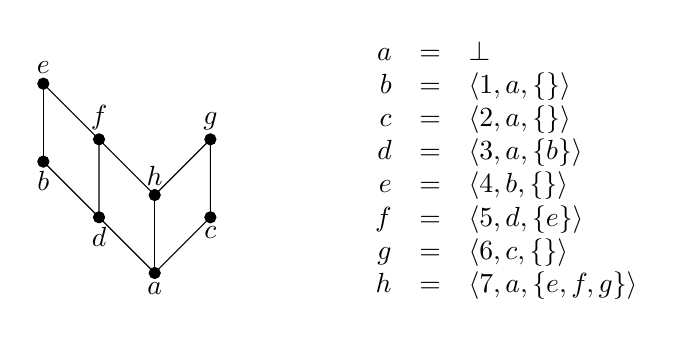
\begin{tikzpicture}
  \begin{scope}[rotate=45]
    \draw (0.0, 2.0) -- (0.0, 0.0) -- (1.0, 0.0);
    \draw (0.0, 2.0) -- (0.7, 2.7);
    \draw (0.7, 2.7) -- (0.7, 1.7);
    \draw (0.0, 1.0) -- (0.7, 1.7);
    \draw (1.0, 0.0) -- (1.7, 0.7);
    \draw (0.7, 1.7) -- (0.7, 0.7) -- (1.7, 0.7);
    \draw (0.0, 0.0) -- (0.7, 0.7);
    \filldraw (0.0, 0.0) circle (2pt) node[below] {$a$};
    \filldraw (0.0, 2.0) circle (2pt) node[below] {$b$};
    \filldraw (1.0, 0.0) circle (2pt) node[below] {$c$};
    \filldraw (0.0, 1.0) circle (2pt) node[below] {$d$};
    \filldraw (0.7, 2.7) circle (2pt) node[above] {$e$};
    \filldraw (0.7, 1.7) circle (2pt) node[above] {$f$};
    \filldraw (1.7, 0.7) circle (2pt) node[above] {$g$};
    \filldraw (0.7, 0.7) circle (2pt) node[above] {$h$};
  \end{scope}
  \draw (2.5, -0.5) node[above right] {
    $\begin{array}{rcl}
    a & = & \bot \\
    b & = & \langle 1, a, \{ \} \rangle \\
    c & = & \langle 2, a, \{ \} \rangle \\
    d & = & \langle 3, a, \{b\} \rangle \\
    e & = & \langle 4, b, \{ \} \rangle \\
    f & = & \langle 5, d, \{e\} \rangle \\
    g & = & \langle 6, c, \{ \} \rangle \\
    h & = & \langle 7, a, \{e,f,g\} \rangle
    \end{array}$
  };
\end{tikzpicture}
\end{center}
\caption{\label{fig:encoding} Embedding elements of $P_3$ into the
  universal domain basis.}
\end{figure}

Figure~\ref{fig:encoding} shows how this system works for embedding
all the elements from the poset $P_3$ into the basis datatype.  The
elements have letter names from $a$--$h$, assigned alphabetically by
insertion order.  In the datatype encoding of each element, the
subordinate and superiors are selected from the set of previously
inserted elements.  Serial numbers are assigned sequentially.

The serial number is necessary to distinguish multiple values that are
inserted in the same position.  For example, in
Fig.~\ref{fig:encoding}, elements $b$ and $c$ both have $a$ as the
subordinate, and neither has any superiors.  The serial number is the
only way to tell such values apart.

Note that the basis datatype seems to contain some junk---some
subordinate/superiors combinations are not well formed.  For example, in
any valid increment, all of the superiors are positioned above the
subordinate.  One way to take care of this requirement would be to
define a well-formedness predicate for basis elements.  However, it
turns out that it is possible (and indeed easier) to simply ignore any
invalid elements.  In the set of superiors, only those values that are
above the subordinate will be considered.  (This will be important to
keep in mind when we define the basis ordering relation.)

There is also a possibility of multiple representations for the same
value.  For example, in Fig.~\ref{fig:encoding} the encoding of $h$ is
given as $\langle 7, a, \{e,f,g\} \rangle$, but the representation
$\langle 7, a, \{f,g\} \rangle$ would work just as well (since the
sets have the same upward closure).  One could consider having a
well-formedness requirement for the set of superiors to be
upward-closed.  But this turns out not to be necessary, since the
extra values do not cause problems for any of the formal proofs.

\subsection{Basis ordering relation}

To perform the ideal completion, we need to define a preorder relation
on the basis.  The basis value $\langle i, a, S \rangle$ should fall
above $a$ and below all the values in set $S$ that are above $a$.
Accordingly, we define the relation ($\preceq$) as the smallest
reflexive, transitive relation that satisfies the following two
introduction rules:
\begin{align}
\label{eq:preceq-1}
a \preceq \langle i, a, S \rangle \\
\label{eq:preceq-2}
a \preceq b \wedge b \in S \Longrightarrow
  \langle i, a, S \rangle \preceq b
\end{align}

Note that the relation ($\preceq$) is not antisymmetric.  For example,
we have both $a \preceq \langle i, a, \{a\} \rangle$ and $\langle i,
a, \{a\} \rangle \preceq a$.  However, for ideal completion this does
not matter.  Basis values $a$ and $\langle i, a, \{a\} \rangle$
generate the same principal ideal, so they will be identified as
elements of the universal domain.

Also note the extra hypothesis $a \preceq b$ in
Eq.~(\ref{eq:preceq-2}).  Because we have not banished ill-formed
subordinate/superiors combinations from the basis datatype, we must
explicitly consider only those elements of the set of superiors that
are above the subordinate.

\subsection {Building the Embedding and Projection}

In the HOLCF formalization, the embedding function \emph{emb} from $D$
to $U$ is defined using continuous extension.  The first step is to
define \emph{emb} on basis elements, generalizing the pattern shown in
Fig.~\ref{fig:encoding}.  The definition below uses wellfounded
recursion---all recursive calls to \emph{emb} are on previously
inserted values with smaller \emph{place} numbers:
\begin{align}
\mathit{emb}(x) & =
\begin{cases}
\bot & \mbox{if}~x = \bot \\
\langle i, a, S \rangle & \mbox{otherwise}
\end{cases} \notag \\
\mbox{where}~i & = \mathit{place}(x) \label{eq:emb} \\
a & = \mathit{emb}(\mathit{sub}(x)) \notag \\
S & = \{\mathit{emb}(y) \mid \mathit{place}(y) < \mathit{place}(x)
\wedge x \sqsubseteq y\} \notag
\end{align}
The subordinate value $a$ is computed using a helper function
\emph{sub}, which is defined as $\mathit{sub}(x) =
\mathit{approx}_{n-1}(x)$, where $n = \mathit{rank}(x)$.  The ordering
produced by the \emph{place} function ensures that no previously
inserted value with the same rank as $x$ will be below $x$.  Therefore
the previously inserted value immediately below $x$ must be
$\mathit{sub}(x)$, which comes from the previous rank.

In order to complete the continuous extension, it is necessary to prove
that the basis embedding function is monotone.  That is, we must show
that for any $x$ and $y$ in the basis of $D$, $x \sqsubseteq y$
implies $\mathit{emb}(x) \preceq \mathit{emb}(y)$.  The proof is by
well-founded induction over the maximum of $\mathit{place}(x)$ and
$\mathit{place}(y)$.  There are two main cases to consider:
\begin{itemize}
\item Case $\mathit{place}(x) < \mathit{place}(y)$: Since $x
  \sqsubseteq y$, it must be the case that $\mathit{rank}(x) <
  \mathit{rank}(y)$.  Then, using the definition of \emph{sub} it can
  be shown that $x \sqsubseteq \mathit{sub}(y)$; thus by the inductive
  hypothesis we have $\mathit{emb}(x) \preceq
  \mathit{emb}(\mathit{sub}(y))$.  Also, from Eq.~(\ref{eq:preceq-1})
  we have $\mathit{emb}(\mathit{sub}(y)) \preceq \mathit{emb}(y)$.
  Finally, by transitivity we have $\mathit{emb}(x) \preceq
  \mathit{emb}(y)$.

\item Case $\mathit{place}(y) < \mathit{place}(x)$: From the
  definition of \emph{sub} we have $\mathit{sub}(x) \sqsubseteq x$.
  By transitivity with $x \sqsubseteq y$ this implies $\mathit{sub}(x)
  \sqsubseteq y$; therefore by the inductive hypothesis we have
  $\mathit{emb}(\mathit{sub}(x)) \preceq \mathit{emb}(y)$.  Also,
  using Eq.~(\ref{eq:emb}), we have that $\mathit{emb}(y)$ is one of
  the superiors of $\mathit{emb}(x)$.  Ultimately, from
  Eq.~(\ref{eq:preceq-2}) we have $\mathit{emb}(x) \preceq
  \mathit{emb}(y)$.
\end{itemize}

The projection function \emph{prj} from $U$ to $D$ is also defined
using continuous extension.  The action of \emph{prj} on basis
elements is specified by the following recursive definition:
\begin{equation}
\mathit{prj}(a) =
\begin{cases}
\mathit{emb}^{-1}(a) & \mbox{if}~\exists x.~\mathit{emb}(x) = a \\
\mathit{prj}(\mathit{subordinate}(a)) & \mbox{otherwise}
\end{cases}
\label{eq:prj}
\end{equation}

To ensure that \emph{prj} is well-defined, there are a couple of
things to check.  First of all, the recursion always terminates: In
the worst case, repeatedly taking the subordinate of any starting
value will eventually yield $\bot$, at which point the first branch
will be taken since $\mathit{emb}(\bot) = \bot$.  Secondly, note that
$\mathit{emb}^{-1}$ is uniquely defined, because $\mathit{emb}$ is
injective.  Injectivity of \emph{emb} is easy to prove, since each
embedded value has a different serial number.

Just like with \emph{emb}, we also need to prove that the basis
projection function \emph{prj} is monotone.  That is, we must show
that for any $a$ and $b$ in the basis of $U$, $a \preceq b$ implies
$\mathit{prj}(a) \sqsubseteq \mathit{prj}(b)$.  Remember that the
basis preorder ($\preceq$) is an inductively defined relation;
accordingly, the proof proceeds by induction on $a \preceq b$.
Compared to the proof of monotonicity for \emph{emb}, the proof for
\emph{prj} is relatively straightforward; details are omitted here.

Finally, we must prove that \emph{emb} and \emph{prj} form an ep-pair.
The proof of $\mathit{prj} \circ \mathit{emb} = \mathrm{Id}_D$ is
easy: Let $x$ be any value in the basis of $D$.  Then using
Eq.~(\ref{eq:prj}), we have $\mathit{prj}(\mathit{emb}(x)) =
\mathit{emb}^{-1}(\mathit{emb}(x)) = x$.  Finally, since the equation
is an admissible predicate on $x$, this is sufficient to show that it
holds for all values in the ideal completion.

The proof of $\mathit{emb} \circ \mathit{prj} \sqsubseteq
\mathrm{Id}_U$ takes a bit more work.  As a lemma, we can show that
for any $a$ in the basis of $U$, $\mathit{prj}(a)$ is always equal to
$\mathit{emb}^{-1}(b)$ for some $b \preceq a$ that is in the range of
\emph{emb}.  Using this lemma, we then have
$\mathit{emb}(\mathit{prj}(a)) = \mathit{emb}(\mathit{emb}^{-1}(b)) =
b \preceq a$.  Finally, using admissibility, this is sufficient to
show that $\mathit{emb}(\mathit{prj}(a)) \sqsubseteq a$ for all $a$ in
$U$.

To summarize the results of this section: We have formalized a type
$U$, and two polymorphic continuous functions \emph{emb} and
\emph{prj}.  For any omega-bifinite domain $D$, \emph{emb} and
\emph{prj} form an ep-pair that embeds $D$ into $U$.  The full proof
scripts are available as part of recent developer versions of the
Isabelle, in the theory file \texttt{src/HOLCF/Universal.thy}.

\section{\label{sec:package}Integration with the Domain Package}

There are several remaining steps involved in building a new domain
package that uses the universal domain $U$.
\begin{enumerate}
\item Define a type $T$ consisting of all the deflations over $U$
  whose image sets are omega-bifinite cpos.  Each \emph{value} of type
  $T$ represents a \emph{type}.  Note that the type $T$ is itself a
  cpo; this is important because it lets us use a fixed-point
  combinator to define recursive values of type $T$, representing
  recursive types.

\item For each of the basic type constructors in HOLCF, define a
  deflation combinator as a continuous function over type $T$.  There
  will be combinators for cartesian product, continuous function
  space, strict sums and products, lifting, and basic types like
  \emph{unit} and \emph{bool}.  Combinators for powerdomains could
  also be defined.
  \begin{align*}
  \times_T, \rightarrow_T, \oplus_T, \otimes_T
    & :: T \rightarrow T \rightarrow T \\
  \mbox{lift}_T & :: T \rightarrow T \\
  \mbox{unit}_T, \mbox{bool}_T, \mbox{int}_T & :: T
  \end{align*}

\item Use the deflation combinators, together with a least fixed-point
  operator, to define deflations for recursive types.  For example,
  the \texttt{BoolList} type used earlier should be a solution to the
  domain equation $D \cong \mbox{unit}_T \oplus_T (\mbox{bool}_T
  \otimes_T D)$.  Accordingly, it should be defined using the least
  fixed-point combinator as $\mu D.\ \mbox{unit}_T \oplus_T
  (\mbox{bool}_T \otimes_T D)$.

\item Define each actual recursive type as the image set of its
  corresponding deflation.  The isomorphism and induction rules
  (generated as axioms in the current implementation) will be derived
  from the fixed-point properties.

\item For each newly-defined recursive type (or type constructor),
  keep track of its deflation (or deflation combinator) for use in
  defining other datatypes.

\end{enumerate}

Some of the above items have been formalized in previous work with
Matthews and White \cite{huffman05axiomatic}, but not in the context
of omega-bifinite cpos.

A complete implementation of the design described above would allow
users to define many interesting datatypes that are not currently
supported.  Examples include uses of indirect recursion through
previously-defined datatypes, and also through type constructors
defined outside the domain package, like powerdomains.  Other examples
include datatypes with negative recursion, like the continuation-based
\texttt{Resumption} datatype from the introduction.

This brings us back to the questions about the \texttt{Resumption}
type posed in the introduction.  The induction rule in
Eq.~(\ref{eq:induction}) can be derived from the fixed-point induction
rule for the deflation used to model type \texttt{Resumption r a}.
Due to the indirect recursion, the deflation for type
\texttt{Resumption r a} is defined in terms of the deflation
combinator for type \texttt{Cont r}.  Furthermore, the deflation
combinator happens to coincide with the function \texttt{mapCont},
which explains its appearance in Eq.~(\ref{eq:induction}).  (This is
similar to how the function \texttt{map} doubles as the deflation
combinator for lists.  In general, a map function that satisfies the
functor laws will coincide with the deflation combinator for that
type.)

\section{\label{sec:related}Related Work}

An early example of the purely definitional approach to defining
datatypes is described by Melham, in the context of the HOL theorem
prover \cite{melham89automating}.  Melham defines a type
$(\alpha)\mathit{Tree}$ of labelled trees, from which other recursive
types are defined as subsets.  The design is similar in spirit to the
one presented in this paper---types are modeled as values, and
abstract axioms that characterize each datatype are proved as
theorems.  The main differences are that it uses ordinary types
instead of bifinite domains, and ordinary subsets instead of
deflations.

The Isabelle/HOL datatype package uses a design very similar to the
HOL system.  The type $\alpha~\mathit{node}$, which was originally
used for defining recursive types in Isabelle/HOL, was introduced
by Paulson \cite{paulson97mechanizing}; it is quite similar to the HOL
system's $(\alpha)\mathit{Tree}$ type.  Gunter later extended the
labelled tree type of HOL to support datatypes with arbitrary
branching \cite{gunter94broader}.  Berghofer and Wenzel used a
similarly extended type to implement Isabelle's modern datatype
package \cite{bw99inductivedatatypes}.

The Coq theorem prover takes an alternative approach to defining
datatypes.  Unlike Isabelle or the HOL system, the semantics of
datatypes in Coq are not formalized within the prover itself.  The
rules and limitations for inductive datatype definitions in Coq are
determined outside the logic, as described by Paulin-Mohring
\cite{paulinmohring93}.  However, compared to Isabelle or HOL, Coq
supports many more of the kinds of recursive datatypes found in
Haskell, including higher-order and non-regular datatypes.  The
semantics of such datatypes in Coq will be relevant if the domain
package is ever extended to support them.

On the domain theory side, various publications by Gunter
\cite{gunter85thesis,gunter87universal,gunter92semantics} were the
primary sources of ideas for my universal domain construction.  The
construction of the sequence of increments in
Section~\ref{sec:construction} is just as described by Gunter
\cite[\S5]{gunter87universal}.  However, the use of ideal completion
is original---Gunter defines the universal domain using a colimit
construction instead.  Given a cpo $D$, Gunter defines a type $D^+$
that can embed any increment from $D$ to $D'$.  The universal domain
is then defined as a solution to the domain equation $D = D^+$.  The
construction of $D^+$ is similar to my \texttt{Basis} datatype, except
that it is non-recursive and does not include serial numbers.

Amadio and Curien \cite{amadio+curien} describe how to construct a
model for Type:Type using a universal bounded-complete domain.  The
same method should work for omega-bifinite domains as well: Since the
type $T$ of deflations over $U$ is itself omega-bifinite, type $T$
contains a value that represents type $T$.  This offers the possibility
of modeling higher-rank polymorphism in HOLCF.

\section{\label{sec:conclusion}Conclusion and Future Work}

The Isabelle/HOLCF library of domain theory now provides a universal
domain type, into which any omega-bifinite domain can be embedded.
The set of deflations over the universal domain includes
representations for a large class of recursive datatypes; thus it
forms a suitable starting point for building a purely definitional
datatype package for HOLCF.

Planned future work consists primarily of implementing the domain
package design outlined in Section~\ref{sec:package}.  Other possible
areas for future work involve exploring limitations in the
current design:

\begin{itemize}

\item \emph{Higher-order type constructors.} Higher-order types can be
  represented by deflation combinators with types like $(T \rightarrow
  T) \rightarrow T$.  The problem is that Isabelle's type system only
  supports first-order types.  Although, see \cite{huffman05axiomatic}
  for an admittedly complicated workaround.

\item \emph{Non-regular (nested) datatypes} \cite{bird98nested}.
  Deflation combinators for non-regular datatypes can be defined by
  taking least fixed points at type $T \rightarrow T$, rather than
  type $T$.  Isabelle's type system can also handle the types of the
  constructors.  The problem is that since Isabelle does not support
  type quantification or polymorphic recursion, induction rules and
  recursive functions could not be defined in the normal way.
  However, even if the normal automation is not available, it might
  make sense to support such datatypes in HOLCF; users could define
  and prove things manually by unfolding the definitions.

\item \emph{Higher-rank polymorphism.}  This is not supported by
  Isabelle's type system.  However, the universal domain $U$ could be
  used to model such types, using the construction described by Amadio
  and Curien \cite{amadio+curien}.

\item \emph{Generalized abstract datatypes (GADTs).}  These are
  usually modeled in terms of some kind of type equality constraints.
  For example, type equality constraints are a central feature of
  System F$_\mathrm{C}$ \cite{system-fc}, which models the internal
  representation of Haskell programs used by the Glasgow Haskell
  Compiler (GHC).  But to the extent of this author's knowledge, there
  is no way to model type equality constraints using deflations.

\end{itemize}

\paragraph{Acknowledgments.}
I would like to thank my advisor, John Matthews, for many encouraging
discussions about HOLCF and domain theory, and also for suggesting the
example used in the introduction.  Thanks also to James Hook for
reading drafts and providing helpful comments.

\bibliographystyle{plain}
\bibliography{tphols09}

\end{document}
